\documentclass[11pt,letterpaper]{article}
\usepackage{style/naaclhlt2015}
\usepackage{times}
\usepackage{mdwlist}
\usepackage{hyperref}
\usepackage{graphicx}
\usepackage{latexsym}
\setlength\titlebox{6.5cm} 

\newcommand{\mult}[1]{\mbox{Mult}( #1)}
\newcommand{\dir}[1]{\mbox{Dir}(#1)}
\newcommand{\norm}[2]{\mbox{Norm}\left(#1, #2\right)}

\begin{document}

\begin{center}
{\bf Predicting Betrayal in Online Games}
\noindent\rule{2cm}{0.4pt}
\end{center}

The prisoner's dilemma is elegant in its simplicity: two
prisoners---denied communication---must decide whether to cooperate
with each other or defect.  This foundational thought experiment of
game theory has helped understand many real world scenarios: \dots .
Despite its power, the prisoner's dilemma is woefully unrealistic.
Cooperation and betrayal do not happen in a cell cut off from the rest
of the world.  Instead, real interactions are mediated by
communication: promises are made, then broken, and met with
recriminations.

We propose to study the role of \emph{language} in understanding
betrayal and cooperation in the game of {\bf Diplomacy}.  Diplomacy,
like the prisoner's dilemma, is a repeated game where players choose
to either cooperate or betray other players.  Unlike the prisoner's
dilemma, however, a key component of Diplomacy is \emph{communication}
to convince another player to help you and betray your foes.

Another key difference is that Diplomacy is fun and played around the
world, including over the Internet.  Players communicate with each
other, convincing other players to work with them or betray their
other players.  This provides a valuable source of insight to examine
how people cooperate, compete, and communicate to obtain scarce
resources.

In the rest of this document, we provide a brief overview of
Diplomacy, discuss preliminary results, and outline a novel
probabilistic model to explain and predict the actions of players.

\section{Diplomacy: Communication, Cooperation, and Conflict}

\begin{figure}
  \begin{center}
  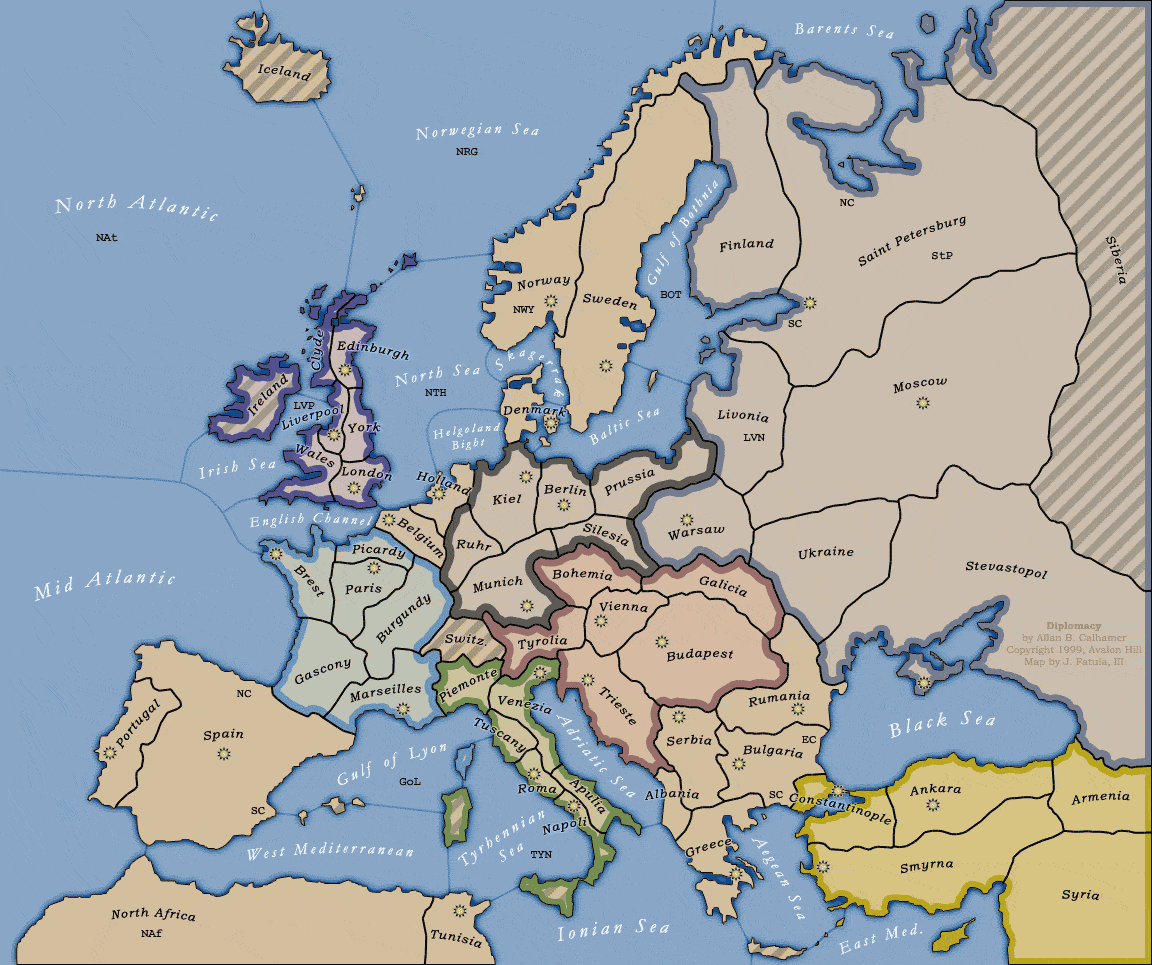
\includegraphics[width=\linewidth]{figures/full_map}
  \end{center}
  \caption{The full Diplomacy board representing Europe circa 1914.
    The seven nations struggle to control the map.}
  \label{fig:board}
\end{figure}

Diplomacy begins in 1914 with players casting themselves as the
European powers at the eve of the first world war: England, Germany,
France, Russia, Austria, Italy, and the Ottoman Empire.  The goal of
the game (like other war games such as Risk or Axis \& Allies) is to
capture all of the territories on the game board
(Figure~\ref{fig:board}).  The game consists of two
phases: \emph{diplomacy} and \emph{orders}.

\subsection{Movement Mechanics}
\label{sec:mechanics}

We begin with the order phase, which is more conventional.  In the
order phase, each of the players writes down their orders for their
units (e.g., a unit can move to an adjacent square if it unoccupied).
A player writes down all of the orders they want to execute.  For
example, Germany may make the following moves:
\begin{itemize*}
        \item army in Berlin moves to Kiel;
        \item army in Munich moves to Ruhr; and
        \item fleet in Kiel moves to Denmark.
\end{itemize*}

The orders for all users are resolved through a set of rules that are
beyond the scope of this document.  The important elements of the game
mechanics are: moves happen simultaneously, there is no randomness,
and ties favor defenders.  To dislodge an opposing force, an attacker
must have numerical superiority.

This is accomplished through units supporting each other.  An adjacent
stationary movement can, in lieu of itself moving, can support the
movement of another unit (Figure~\ref{fig:support}) or support a
stationary unit holding a territory.  Which move succeeds depends on
which side had more support.  For example, a unit holding can be
dislodged by two units (one attacking, another supporting); a unit
holding with the support of another can be dislodged by two units (one
attacking, another supporting, the third either attaching the
supporting unit or supporting the attack).

The nuances of support are important to players, but not particularly
relevant for understanding how people cooperate and compete with each
other.  The key idea is that successful moves need support, and it's
often impossible for a player to act on their own.  They need to get
other players to help them accomplish their goals.  Because these
orders are machine readable, we have a clear indication of when
players are working together (supporting each other) or working
against each other (attacking each other); we will use this to define
a cooperation matrix in Section~\ref{sec:model}.  However,
coordinating these actions between players requires cooperation and
\emph{diplomacy}, which brings us to the second phase of the game.

\subsection{Communication}

In the \emph{diplomacy} phase of the game, players can talk to each
other.  These conversations can either happen globally or---more
typically---one-on-one.  Conversations include greetings, extra-game
discussions (e.g., ``did you see Game of Thrones?''), low-level
strategy (``if you attack Armenia, I'll support you''), high-level
strategy (``we need to capture central Europe'').

As detailed in a recent
\href{http://www.thisamericanlife.org/radio-archives/episode/531/got-your-back?act=1}{\emph{This
    American Life}}, a key component to succeeding in a diplomacy game
is to forge alliances and then break them at the right time.  Thus,
successful play depends on convincing your competitors to support and
help you and then betraying them.

Thus, because of the centrality of language to Diplomacy, we can learn
about the rhetorical and social devices players use to build and break
trust.  Because this language is embedded in a game provides crucial
features: similar situations are repeated, the goals are clear, and
the machine-readable orders let us know who is working with whom and
who are enemies.

In the next section, we describe some preliminary analyses of the the
Diplomacy data.

\section{Preliminary Analysis}

We obtained several hundred complete games of Diplomacy from a two
major online clearing houses for games.  This includes not just the
state of the games but the anonymous communications between players
(all player identities are unknown to both us and their fellow
players).

\subsection{Fundamental Attribution: Winners take credit, losers make excuses}

Success in Diplomacy is measured by the number of supply centers
(cities) that a player holds.  We can use a regression to predict
whether a player increases or decreases their number of supply centers
at the end of a turn.

This regression is presented in Table~\ref{tab:gain-loss}.  To focus
on general language (and not in-game specifics), we show only stop
words (i.e., highly frequent functional words that will appear in any
conversation).

This regression shows that players who are winning focus on team work
and cooperation (``our'' is the highest scoring word), while players
doing less well have pronouns that focus on others (``its'', ``your'',
``their'').  Losing players also focus on the past (``was'') more than
the present (``is'' has higher weight for positive weights).

\begin{table}
  \begin{center}
  \begin{tabular}{cc|cc}
    Weight & Word & Weight & Word \\
    \hline
    +2.3 & our  & -2.2 & also \\
    +1.9 & up   & -2.2 & must \\
    +1.7 & his  & -1.7 & no \\
    +1.5 & an   & -1.6 & any\\
    +1.4 & in   & -1.0 & of\\
    +1.3 & now  & -0.8 & its\\
    +1.2 & for  & -0.8 & was\\
    +1.2 & when & -0.8 & upon\\
    +1.2 & is   & -0.8 & were\\
    +1.2 & there& -0.8 & their\\
    +1.0 & if   & -0.8 & some\\
    +1.0 & by   & -0.7 & may\\
    +1.0 & be   & -0.7 & are\\
    +0.9 & and  & -0.5 & your\\
    +0.9 & down & -0.5 & can\\
    \hline
  \end{tabular}
  \end{center}
  \caption{Predicting gains (positive) or losses (negative) in the game.}
  \label{tab:gain-loss}
\end{table}

\subsection{Perfidy Parity}
\label{sec:parity}

More interesting than how an individual is faring in a game is to look
at the relationships between players.  We define a variable
$y_{ij}^{(t)}$ to encode whether players are friends (+1) or enemies
(-1) during time $t$.  From this we can also define the parity as the
number of sign changes of the sequence of $y_{ij}$ ignore
indeterminate states; for example $\{+1, +1, 0, +1, {\bf -1}\}$ would
have one parity change, while $\{-1, 0, -1, 0, {\bf +1}, +1, {\bf
  -1}\}$ would have two.

Figure~\ref{fig:parity} shows the distribution of parity when two
players are friends at the end of the game.  What is interesting about
this figure is that there are no odd parities; if a player has
betrayed you once, they never ``stay true'' to the end of the game.

Thus, a challenge for players and also for us as researchers is to
predict when pay-back will happen.  Can we predict when one player will
``stab'' (in the lingo of Diplomacy) another?

\begin{figure}[tbh]
  \begin{center}
    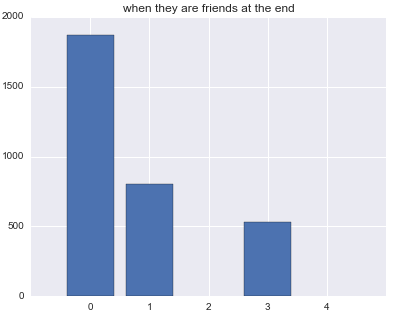
\includegraphics[width=0.9\linewidth]{figures/flip_distribution_split}
    \caption{The parity of relationships in Diplomacy.  Either two
      players remain friends or enemies throughout the game or they
      ``flip'' an odd number of times.}
    \label{fig:parity}
  \end{center}
\end{figure}

\begin{figure*}
  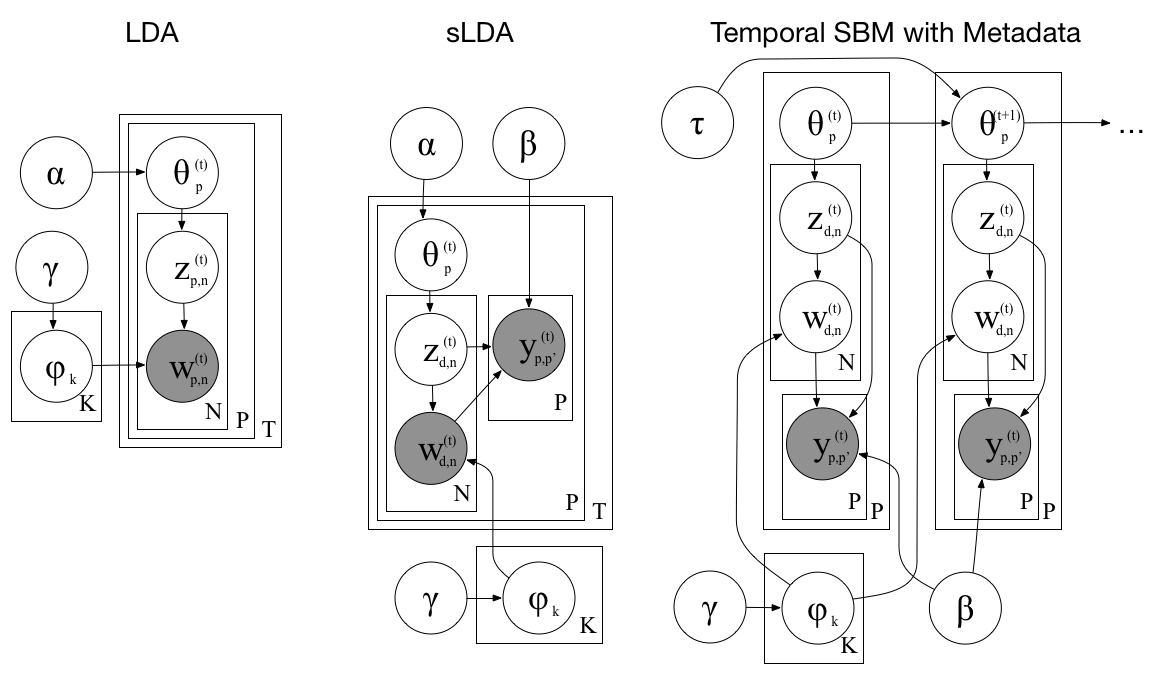
\includegraphics[width=0.9\linewidth]{figures/graphical_model}
  \caption{Models we propose to apply to Diplomacy data}
\end{figure*}

\section{Proposed Model for Understanding Betrayal and Cooperation}
\label{sec:model}

We propose a novel graphical model to capture the evolution of games
and to predict what players will do.  This model combines supervised
prediction with sequential modeling.

We first posit that the words a player utters are described by a
collection of latent topics.  Each player $p$'s communications in a
turn $t$ is described by a topic distribution $\theta^{(t)}_{p}$; this
is a multinomial distribution over topics from which topic assignments
for each token $n$ is drawn $z^{(t)}_{p,n} \sim
\mult{\theta^{(t)}_{p}}$.  Finally, each observed word $w^{(t)}_{p,n}
\sim \mult{\phi_{z^{(t)}_{p,n}}}$, where $\phi$ is a topic's
distribution over words.

Alone, this gives us a clustering of the words players use.  We can
discover words that cooccur together, reflecting geographic (parts of
the board), relationship (friend / foe), temporal (early game / late
game) clusters.

\paragraph{Supervised Model}

However, we are interested in \emph{predicting} whether players will
work together or not.  Do do this, we need to add supervision to the
underlying model.  Thus, we also have a link between pairs of players
$y^(t)_{i,j}$ that encodes whether they are friend ($+1$) or foe ($-1$).
We model these links as
\begin{equation}
y^{(t)}_{i,j} \sim \norm{\bar{z}^{(t)}_{i} \beta \left[ \bar{z}^{(t)}_{j}\right]^{\top}}{\sigma^2},
\end{equation}
where $\beta$ is an affinity matrix that provides the interaction
between the topics in two player's interactions.

\paragraph{Adding Additional Features}

Adding additional features can further improve prediction: adding
word-level and temporal features can help predict whether players will
be friend or foe.  Thus, in addition to the topics that a player uses
in a turn, we can also add features that represent specific words,
aspects of the map, etc.

\paragraph{Temporal Modeling}

Finally, adding temporal models can help capture the evolution of
players' communication patterns by adding the additional constraint
that topics shouldn't change radically over time.  Thus, we can add a
switch variable $\tau_p^{(t+1)}$ that indicates whether a distribution
over topics has changed from time $t$ when player $p$ has a new topic
distribution for a player $\theta_p^{(t)}$.

We have previously used these models to indicate when people change
what they're talking about.  Because of the joint dependence also on
the relationships $y_{ij}$, we also hope that these segments will
capture the subtle shifts in language the can help predict when
players choose to betray each other.

\end{document}
